\section{ClustAssess package}

\subsection{ECS optimization}

\begin{frame}[label=ecs-first]{What is ECS?}
    \begin{itemize}
        \item An \textit{affinity matrix} of a partition summaries the co-occurrences of elements by calculating the number of different paths between them.
        \item  For a disjoint partition, the affinity matrix is calculated using the formula: \begin{equation*} \label{eq:affinity-disjoin}
                  p_{ij} =
                  \begin{cases}
                      0, \text{if } i \text{ and } j \text{ don't belong to the same cluster}                  \\
                      \frac{\alpha}{|C_\beta|}, \text{if }i\text{ and } j \text{ belong to the cluster } \beta \\
                      1 - \alpha + \frac{\alpha}{|C_\beta|}, \text{if } i = j
                  \end{cases}
              \end{equation*}
        \item Element-Centric Similarity (ECS) \cite{Gates2019} is a clustering comparison score built on the L1 distance between the affinity matrices: $ \displaystyle S_i (\mathcal{A}, \mathcal{B}) = 1 - \frac{1}{2 \alpha} \sum_{j = 1}^N |p_{ij}^{\mathcal{A}} - p_{ij}^{\mathcal{B}}|$
    \end{itemize}

    \hyperlink{app1}{\beamerbutton{ECS properties}}

\end{frame}

\begin{frame}[label=optslide]{Optimising the calculation of the ECS score for disjoint partitions}
    \begin{itemize}
        \item For disjoint partitions, the ECS has the same value for points from the same clusters.
        \item The number of ECS calculations drops from $N \times N$ to $n \times m$, where $n$ is the number of clusters of the first partition and $m$ is the number of clusters of the second. 
        \item This optimization removes the dependency on the affinity matrix and enhances the time and memory efficiency.

    \end{itemize}
    
    \hyperlink{proof}{\beamergotobutton{Optimization proof}}
\end{frame}

\begin{frame}{Element-Centric Consistency}
    \begin{itemize}
        \item Gates et al. also proposed Element-Centric Consistency (or ECC; also named  \textit{frustration}) score, used on a list of multiple partitions.
        \item The ECC score is calculated as the average of the sum of the ECSs obtained for every unique pair of partitions from the list:
              \begin{equation*}
                  \frac{2}{T(T-1)} \sum_{j=1}^T \sum_{k=1}^{j-1} S_i (\mathcal{R}_k, \mathcal{R}_j)
              \end{equation*}
    \end{itemize}
\end{frame}


\begin{frame}[label=wecc]{Weighted ECC}
    \begin{itemize}
        \item For multiple occurrences of the same partition, the ECC requires redundant calculations of the ECS of equivalent pairs.
        \item To alleviate the computational burden, we proposed a weighted version of ECC, where for each unique partition we retain a weight that is the number of duplicates.
    \end{itemize}
    \hyperlink{proof}{\beamerbutton{Weighted ECC pseudocode}}
\end{frame}

\begin{frame}{Merging identical partitions}
    \begin{columns}
        \begin{column}{0.45\textwidth}
            \justifying

            The weights are calculated by performing an automatic merge of identical partitions.
            \bigskip

            To determine if two partitions are identical, we use their contingency table.
        \end{column}

        \begin{column}{0.5\textwidth}
            \begin{figure}
                \centering
                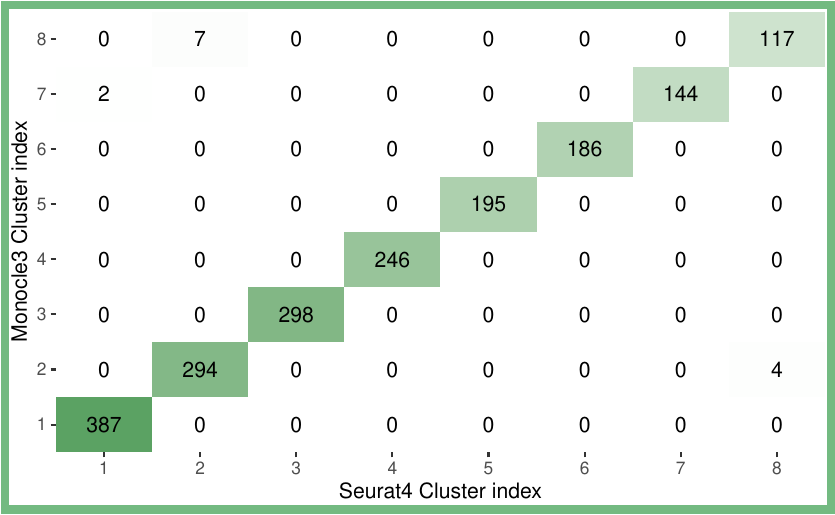
\includegraphics[width=\textwidth]{images/ch2/2_cont_table.png}
                \caption{\justifying \textbf{Pair-wise contingency table}. The rows are associated with the clusters from one partition, and the columns with the clusters from the other partitions. In each $[i,j]$ cell we present the number of cells in clusters $i$ and $j$, respectively}
            \end{figure}
        \end{column}
    \end{columns}
    
\end{frame}
\begin{frame}{Almost identical partitions - ECS threshold}
    There are cases where the difference between two partitions is negligible (see below).
    To allow the merging of almost identical partitions, we introduced the \textit{ECS threhshold} i.e.  a lower bound for the ECS for determining partitions which can be considered quasi identical and merge-able.
    \begin{figure}
        \centering
        \begin{subfigure}[t]{0.47\textwidth}
            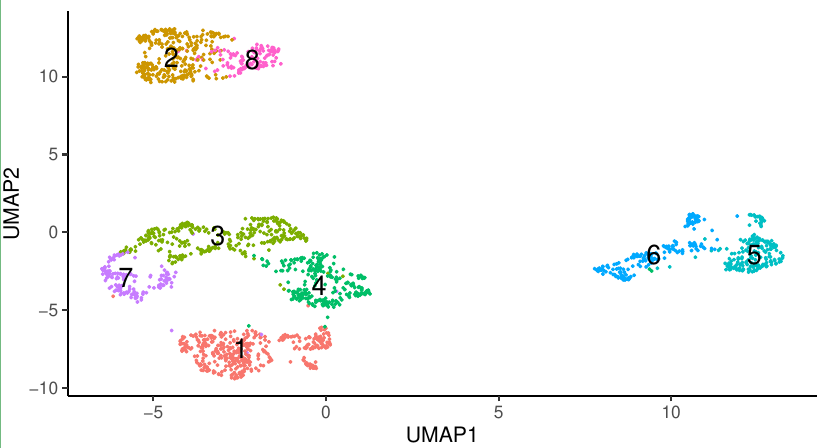
\includegraphics[width=\textwidth]{images/ch2/2_almost_s.png}
        \end{subfigure}
        \begin{subfigure}[b]{0.47\textwidth}
            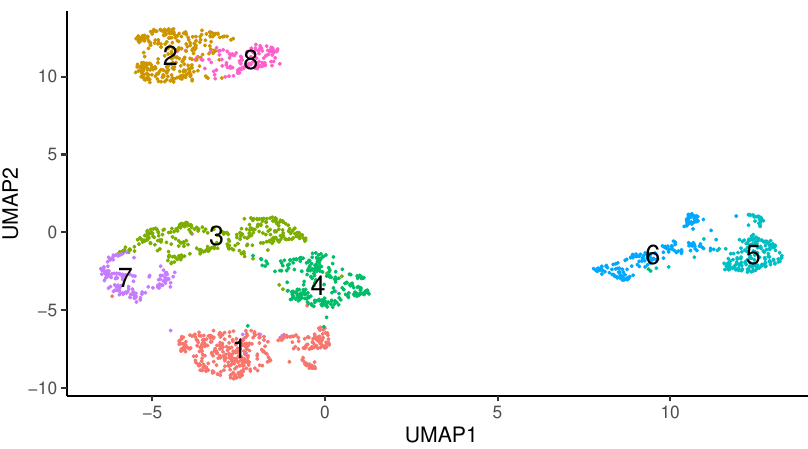
\includegraphics[width=\textwidth]{images/ch2/2_almost_m.png}
        \end{subfigure}
        \caption{\textbf{Two almost identical partitions} Each panel represents the distribution of a partition on a low-dimensional (UMAP) topology.}
    \end{figure}
\end{frame}

\subsection{Stability pipeline}

\begin{frame}
    \begin{itemize}
        \item Random seed is a factor that affects the clustering output.
        \item We developed a stability pipeline that offers a set of visual summaries for the assessment of the robustness of a parameter configuration in the context of variable random seeds.
        \item The robustness is determined by running the clustering pipeline multiple times on different random seeds. The Element-Centric Consistency of the obtained list of partitions is an indicator of stability.
        \item The stability pipeline follows the steps presented in the PhenoGraph algorithm.
    \end{itemize}
\end{frame}

\begin{frame}{Feature stability}
    \begin{columns}
        \begin{column}{0.45\textwidth}
            \justifying

            The feature set has an important role in obtaining the low-dimensional topology.
            \bigskip


            We assess the stability of different feature sets with varying sizes.
            \bigskip


        \end{column}

        \begin{column}{0.5\textwidth}
            \begin{figure}
                \centering
                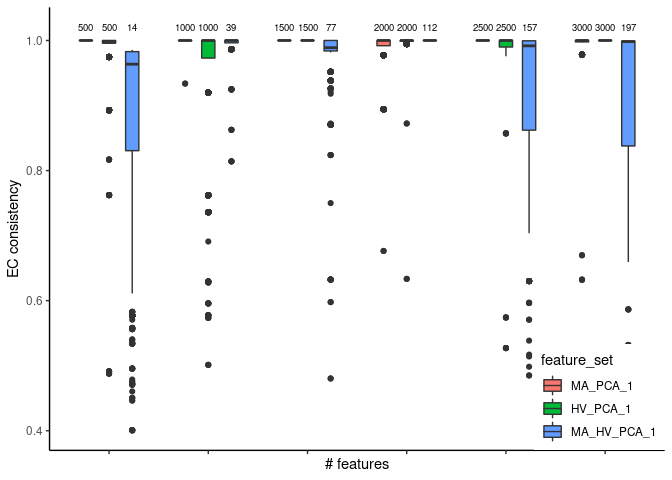
\includegraphics[width=\textwidth]{images/ch3/3_feat_incremental.png}
                \caption{\justifying \textbf{Incremental stability of feature sets}. Each colour corresponds to a different feature set. The size of the set is displayed above each boxplot. Each boxplot represents the ECS distribution across partitions.}
            \end{figure}
        \end{column}
    \end{columns}
\end{frame}

\begin{frame}{The impact of the number of nearest neighbours on the graph connectivity}
    \begin{columns}
        \begin{column}{0.45\textwidth}
            \justifying

            The number of nearest neighbours affects the graph connectivity.
            \bigskip


            The number of connected components decreases as the number of nearest neighbours increases.
            \bigskip

            The number of connected components is a lower bound for the possible number of clusters.


        \end{column}

        \begin{column}{0.5\textwidth}
            \begin{figure}
                \centering
                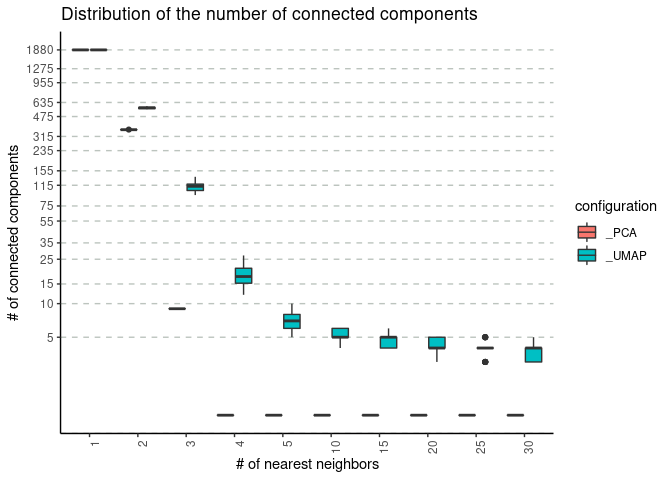
\includegraphics[width=\textwidth]{images/ch3/3_conn_comp.png}
                \caption{\justifying \textbf{Graph connectivity assessment}. The colour indicates the reduced space used for graph building. On the X-axis we vary the number of nearest neighbours. The Y-axis indicates the number of connected components. }
            \end{figure}
        \end{column}
    \end{columns}
\end{frame}


\begin{frame}{Resolution - number of clusters stability}
    \begin{columns}
        \begin{column}{0.45\textwidth}
            \justifying

            For graph clustering methods, the resolution parameter controls the number of clusters.
            \bigskip


            The stability can be assessed on different parameter configurations.
            \bigskip

            The colour gradient describes the statistical reliability of the assessment.


        \end{column}

        \begin{column}{0.5\textwidth}
            \begin{figure}
                \centering
                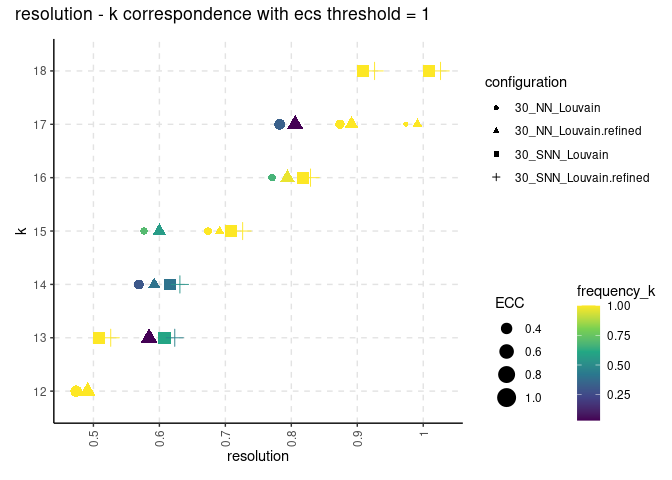
\includegraphics[width=\textwidth]{images/ch3/3_1_kres_ecc.png}
                \caption{\justifying \textbf{Stability link between the Resolution and the number of clusters}. Each point-shape indicates a parameter configuration. The point size quantifies the stability of the resolution - number of clusters pair. The colour gradient illustrates the frequency of the number of clusters.}
            \end{figure}
        \end{column}
    \end{columns}
\end{frame}